\pagestyle{fancy}
\fancyhead[l]{\autorUO}
\fancyfoot[l]{\asignaturaAbbr}
\fancyfoot[r]{\fecha}

\section{Imágenes \textit{RAW}} \label{sec:raw_images}
[...]

\subsection{Lectura de una imagen \textit{RAW}} \label{subsec:raw_image_reading}
\begin{figure}[h]
    \centering
    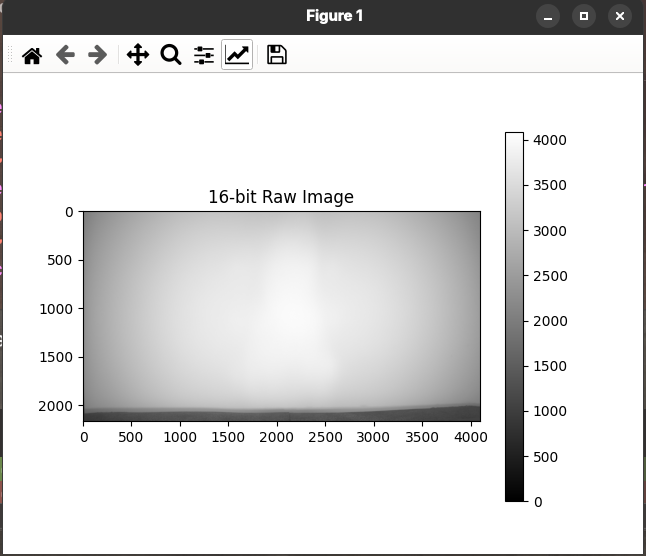
\includegraphics[width=0.55\textwidth]{img/16bit_raw.png}
    \caption{Lectura de una imagen \textit{RAW} utilizando \textit{numpy} y \textit{matplotlib}}
    \label{fig:raw_image_reading}
\end{figure}

\subsection{Mosaico de Bayer} \label{subsec:bayer_mosaic}
[...]

\newpage
\subsection{Módulo \textit{debayer}} \label{subsec:debayer_module}
\begin{figure}[h!]
    \centering
    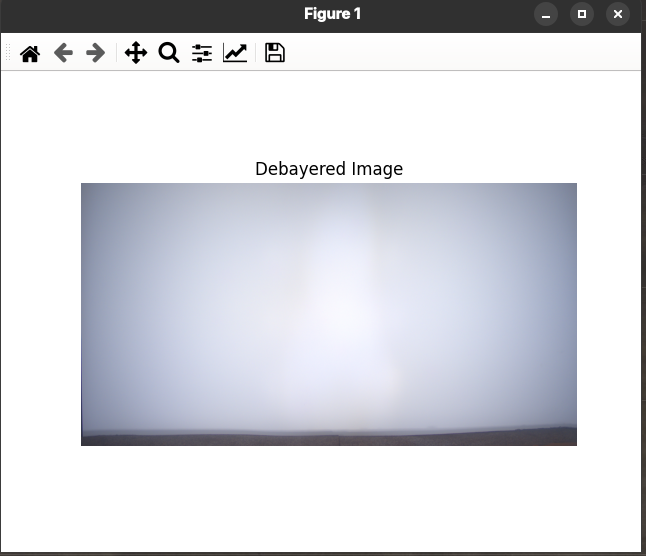
\includegraphics[width=0.55\textwidth]{img/debayered.png}
    \caption{Imagen \textit{RAW} \textit{debayered} utilizando \textit{Debayer5x5}}
    \label{fig:raw_image_debayered}
\end{figure}


\subsection{Mejora del contraste con sigmoides} \label{subsec:sigmoid_contrast_enhancement}
\begin{figure}[h!]
    \centering
    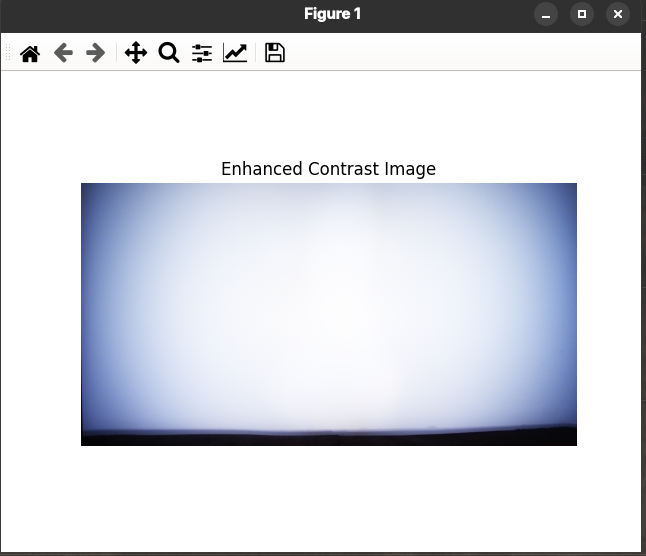
\includegraphics[width=0.55\textwidth]{img/enhanced_contrast.png}
    \caption{Imagen \textit{RAW} tras mejora del contraste con función sigmoide}
    \label{fig:raw_image_sigmoid_contrast}
\end{figure}
